\documentclass[a4paper]{kulakarticle}

\usepackage[utf8]{inputenc}
\usepackage[dutch]{babel}
\usepackage{titling}
\title{Kost van een Airbnb-verblijf}
\author{Project statistiek}
\date{Academiejaar 2022 -- 2023}
\address{
	Louis Vandenbruwaene\\
	Jasper Denorme\\
	Dieter Demunck}
\usepackage{graphicx,flafter,framed,caption}
\usepackage{amsfonts,amssymb,amsmath,textcomp,eurosym,wasysym}
\usepackage{listings}
\usepackage{siunitx}
\sisetup{output-decimal-marker={,}}
\usepackage{enumitem}
\usepackage{multicol}
\usepackage{caption}
\usepackage{tabularx,array}
\newcommand{\rood}[1]{\textcolor{red}{#1}}

\begin{document}
	\maketitle
	\section*{Inleiding}
	Airbnb is een online platform (\href{https://www.airbnb.com}{\texttt{www.airbnb.com}}) waarop reizigers een kort verblijf kunnen boeken in een accommodatie (bv. een kamer, een huis, een woonboot, …) die door particulieren wordt verhuurd. Airbnb werd opgericht in 2008 en is ondertussen een erg populair alternatief geworden voor de traditionele hotels. \\
	
	Dit onderzoek focust op de totale kostprijs voor het huren van een Airbnb-verblijf in Amsterdam voor twee personen gedurende een weekend (vrijdag tot zondag). Er wordt nagegaan met welke factoren deze kostprijs samenhangt en in welke mate de kost daarmee kan worden voorspeld. Hierbij wordt er gebruik gemaakt van een aantal veranderlijken verzameld in het kader van een onderzoeksproject uitgevoerd door Kristóf Gyódi en Łukasz Nawaro. Het gaat enerzijds over kenmerken van het verblijf en tevredenheid van eerdere gasten volgens de gegevens van Airbnb, anderzijds over de ligging van het verblijf ten opzichte van het stadscentrum, bezienswaardigheden en restaurants, telkens rekening houdend met de populariteit, zoals gerapporteerd door TripAdvisor.\\
	
	Tabel \ref{beschrijving} beschrijft de variabelen en tabel \ref{uitreksel} geeft enkele basisstatistieken weer van de veranderlijken die gebruikt worden in het onderzoek. \\\\

\begin{table}[h]
	\centering
	\begin{tabular}{c|p{10cm}}
		\raggedright
		Naam & Beschrijving\\
		\hline
		realSum & Som van alle kosten in euro\\ 
		room & Soort verblijf (1 = volledige woning, 2 = afzonderlijke kamer, 
		3 = gedeelde kamer) \\ 
		capacity & Maximaal aantal gasten \\
		bedrooms & Aantal beschikbare slaapkamers in het verblijf \\
		dist & Aantal beschikbare slaapkamers in het verblijf (km) \\
		metro & Afstand tot dichtstbijzijnde metro-halte (km)\\
		attr & Attractiescore, nabijheid van bezienswaardigheden \\
		rest & Restaurantscore, nabijheid van restaurants \\ 
		host & Type verhuurder (0 = enige beschikbare woning, 1 = 2 tot 4 beschikbare woningen,
		2 = meer dan 4 beschikbare woningen) \\ 
		cleanliness & Modale score voor netheid van het verblijf volgens gasten (op 10) \\
		satisfaction & Tevredenheid van de gasten (op 10)\\
		
	\end{tabular}
	\caption{Beschrijving van de gebruikte veranderlijken.}
	\label{beschrijving}
\end{table}
\begin{table}[h]
	\centering
	\begin{tabular}{| l| l| l|  p{5cm} |}
		\hline
		Naam & Gemiddelde $\pm$ standaardfout  & Bereik & Algemene vorm\\  [1ex]
		\hline\hline
		realSum & $604.8\pm 443.6828 $ & $7964.755$  &  zeer rechtsscheef\\    [0.5ex]
		\hline
		capacity & $2.77\pm 1.019876$ & $4$  & rechtsscheef \\[0.5ex]
		\hline
		bedrooms & $1.303\pm 0.7329492$ & $5$ & rechtsscheef \\[0.5ex]
		\hline
		dist & $2.80634\pm 2.036602$  & $11.18089$ & zeer rechtsscheef \\  [0.5ex]
		\hline
		metro & $1.0892\pm 0.8265551$ & $4.375388$ & zeer rechtsscheef \\ [0.5ex]
		\hline
		attr & $2.101\pm 0.9407762$ & $9$  & rechtsscheef \\  [0.5ex]
		\hline
		rest & $3.285\pm 1.760009$ & $9$ & benaderend lognormaal met zware staarten \\ [0.5ex]
		\hline
		cleanliness & $9.471\pm 0.8306492$ & $8$ & benaderend exponentieel  \\ [0.5ex]
		\hline
	\end{tabular}
	\caption{Basisstatistieken van de gebruikte veranderlijken.}
	\label{uitreksel}
\end{table}
	
	\section{Methode}
	\rood{Deze sectie telt hoogstens één pagina (exclusief figuren en tabellen).}
	\subsection{Kenmerken van de steekproef}
Om te testen of de gemiddelde kost veranderd is tegenover 2019, maken we gebruik van een student t-test voor één gemiddelde. We mogen deze gebruiken, want de dataset voldoet aan de centrale limietstelling (n = 977). Om na te gaan of het aandeel particuliere verhuurders groter is dan het aantal professionele verhuurders, hebben we van een $z$-test voor één proportie gebruikt.\\
 
 We zijn via een $\chi ^2$-test nagegaan of het aantal beschikbare kamers Poisson verdeeld is. Dit deden we nadat we data bij elkaar hebben gegooid, om aan de Cochranregel te voldoen.
	
	\subsection{Gemiddelde kost}
	
	Hier zal onderzocht worden of de totale prijs van een verblijf voor twee personen afhankelijk is van andere variabelen. Ten eerste 
	

	\subsection{Associatie met de verschillende veranderlijken}
	

	Verder wordt de associatie tussen \textbf{realsum} en de andere veranderlijken onderzocht. Aangezien \textbf{realsum} niet normaal verdeeld is (zie figuur \ref{fig:clean1}) en er zelden samenvallende waarden voorkomen, wordt getest of de Spearman rangcorrelatie van de prijs met de continue variabelen significant van nul verschilt. Om de afhankelijkheid met de discrete en kwalitatieve variabelen te bepalen, wordt een $\chi ^2$-test gebruikt. Hiervoor wordt gewerkt met de gediscretiseerde \textbf{realsum}. Ook de discrete en kwalitatieve variabele worden samengevoegd om zo goed mogelijk aan de Cochranregel te voldoen. Enkel \textbf{host} blijft onveranderd. \textbf{Realsum} wordt verdeeld volgens zijn $4$ kwantielen en de andere opdelingen zijn te vinden in tabel \ref{grenzen}\\\\
	\begin{table}[h]
		\centering
			\begin{tabular}{c|c}
			\centering
			naam& opdelende grenzen\\
			\hline
			\textbf{cleanliness} & $ 0 $ - $ 7.5 $ - $ 8.5$ - $ 9.5 $ - $ 10.5$ \\
			\textbf{capacity}& $-0.5$ - $2.5$ - $3.5$ - $4.5$ - $6.5$\\
			\textbf{bedrooms}& $-0.5$ - $0.5$ - $1.5$ - $2.5$ - $6$\\
			\textbf{room} & $0.5$ - $1.5$ - $3.5$\\
			\end{tabular}
			\caption{De grenzen, die de gegevens opdelen zodat de aan Cochran-regel voldaan is.}
			\label{grenzen}
	\end{table}
	\subsection{Verklaren van de kost}
	
	
	\section{Resultaten}
	\rood{Deze sectie telt hoogstens één pagina (exclusief figuren en tabellen).}
	\subsection{Kenmerken van de steekproef}
De gemiddelde kost in de steekproef is 604 euro, terwijl deze in 2019 620 euro was. Het verschil van 16 euro is niet significant ($t_{976}$ = -1.1, p = 0.29). We kregen $\chi^2 = 89.074$ en $p \approx 0$ voor onze test op het aandeel van particuliere vs. professionele verhuurders. We bekomen een verschil van 295. Bij de $\chi$-kwadraat test voor onze verdeling bekomen we $\chi^2 = 424.77$ en $p \approx 0$, we kunnen dus aannemen dat het aantal beschikbare kamers niet Poisson verdeeld is.
	\subsection{Gemiddelde kost}
	
	
	
	\subsection{Associatie met de verschillende veranderlijken}
	
	Uit tabel \ref{continue variabelen afhankelijkheid} kunnen we met aan zekerheid grenzende waarschijnlijkheid concluderen dat \textbf{realsum} afhankelijk is van elke continue variabele in de dataset. De bijhorende correlatie wordt geschat door rho.
	\begin{table}
		\begin{tabular}{c|c|c|c }
			naam & p-waarde & afhankelijkheid & rho\\
			\hline
			\hline
			dist & $< 2.2 \cdot 10^{-16} $&ja& $-0.4107378$ \\
			metro &$ 9.476\cdot 10^{-10}$& ja& $-0.1941159$ \\ 
			attr &$ < 2.2\cdot 10^{-16}$& ja&$0.4314979 $ \\
			rest &$ < 2.2\cdot 10^{-16}$& ja&$0.4276987 $ \\
			satisfaction &$ 1.657\cdot 10^{-7}$& ja&$0.1664983 $ \\
		\end{tabular}
		\caption{Afhankelijkheid van de prijs met de continue variabelen.}
		\label{continue variabelen afhankelijkheid}
	\end{table}
	Uit tabel \ref{discrete variabelen afhankelijkheid} kunnen we met aan zekerheid grenzende waarschijnlijkheid besluiten dat \textbf{realsum} afhankelijk is van: \textbf{capacity}, \textbf{bedrooms}, \textbf{room} en \textbf{host}. We kunnen ook met grote waarschijnlijkheid zeggen dat \textbf{cleanliness} niet gecorreleerd is met \textbf{realsum}. 
	\begin{table}[h]
		\begin{tabular}{c|c|c|c }
			naam & p-waarde & afhankelijkheid & $\chi ^2$\\
			\hline
			\hline
			cleanliness & $0.7775$&nee& $5.6174$ \\
			capacity &$ < 2.2\cdot 10^{-16}$& ja& $390.3$ \\ 
			bedrooms &$ < 2.2\cdot 10^{-16}$& ja&$368.1 $ \\
			room &$ < 2.2\cdot 10^{-16}$& ja&$ 337.29$ \\
			host &$ 5.506\cdot 10^{-7}$& ja&$39.581 $ \\
		\end{tabular}
		\caption{Afhankelijkheid van de prijs met de discrete en kwalitatieve variabelen.}
		\label{discrete variabelen afhankelijkheid}
	\end{table}
	
	
	
	\subsection{Verklaren van de kost}
	Lorem ipsum dolor sit amet, consectetur adipiscing elit, sed do eiusmod tempor incididunt ut labore et dolore magna aliqua. Ut enim ad minim veniam, quis nostrud exercitation ullamco laboris nisi ut aliquip ex ea commodo consequat. Duis aute irure dolor in reprehenderit in voluptate velit esse cillum dolore eu fugiat nulla pariatur. Excepteur sint occaecat cupidatat non proident, sunt in culpa qui officia deserunt mollit anim id est laborum.
	
	Lorem ipsum dolor sit amet, consectetur adipiscing elit, sed do eiusmod tempor incididunt ut labore et dolore magna aliqua. Ut enim ad minim veniam, quis nostrud exercitation ullamco laboris nisi ut aliquip ex ea commodo consequat. Duis aute irure dolor in reprehenderit in voluptate velit esse cillum dolore eu fugiat nulla pariatur. Excepteur sint occaecat cupidatat non proident, sunt in culpa qui officia deserunt mollit anim id est laborum.
	
	\section{Discussie}
	\rood{Deze sectie telt hoogstens één pagina (exclusief figuren en tabellen).}
	\subsection{Kenmerken van de steekproef}
Op basis van de steekproef lijkt er geen verandering te zijn in de kostprijs van een kamer. Met aan zekerheid grenzende waarschijnlijkheid kunnen we aannemen dat er meer particulier verhuurders zijn, het lijkt er dus op dat er een 'strenge' regulering is in Amsterdam. We kunnen ook met zeer grote waarschijnlijkheid aannemen dat het aantal beschikbare kamers niet Poisson verdeeld is.
	
	\subsection{Gemiddelde kost}
	
	\subsection{Associatie met de verschillende veranderlijken}
	
	Op basis van de steekproef zijn \textbf{attr}, \textbf{rest}, \textbf{capacity}, \textbf{room}, \textbf{host}, \textbf{bedrooms} en \textbf{satisfaction} positief gecorreleerd met \textbf{realsum}. Bij de continue variabelen kunnen we dit afleiden uit de rho en bij de andere kunnen enkel kijken naar de scatterplots. Daarentegen zijn \textbf{dist} en \textbf{metro} negatief gecorreleerd met de totale prijs. Dit is duidelijk uit de waarde van rho. Intuïtief is dit ook aanvaardbaar. Toegankelijkheid tot het stadscentrum en een metrohalte verhoogt de waarde van een verblijf.
	
\begin{figure}
	\centering
	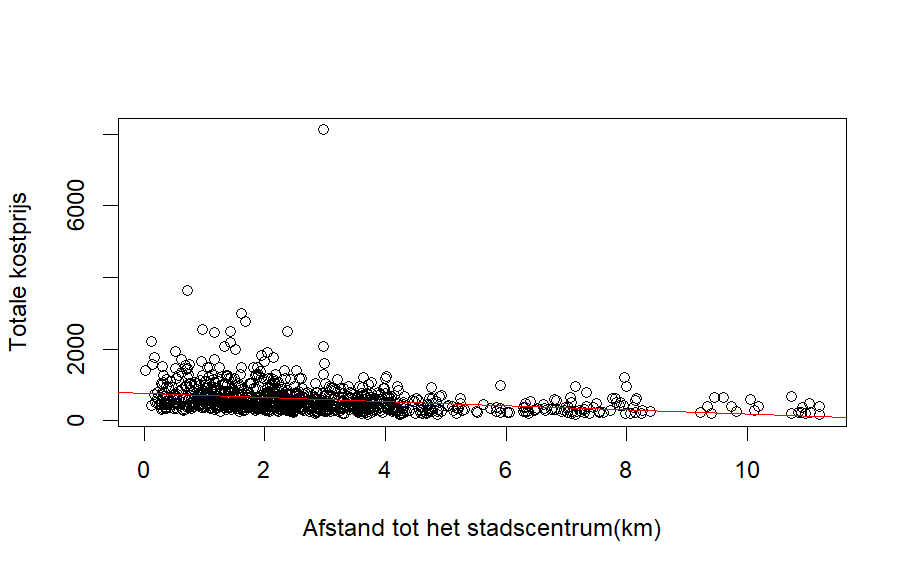
\includegraphics[width=0.49\linewidth]{../../../../Pictures/project.stat/dist}
	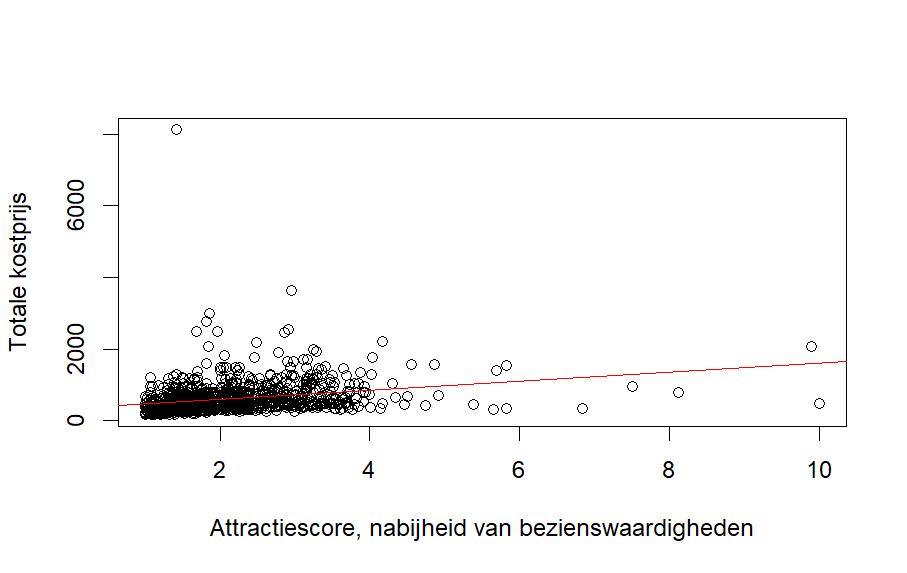
\includegraphics[width=0.49\linewidth]{../../../../Pictures/project.stat/attr}
	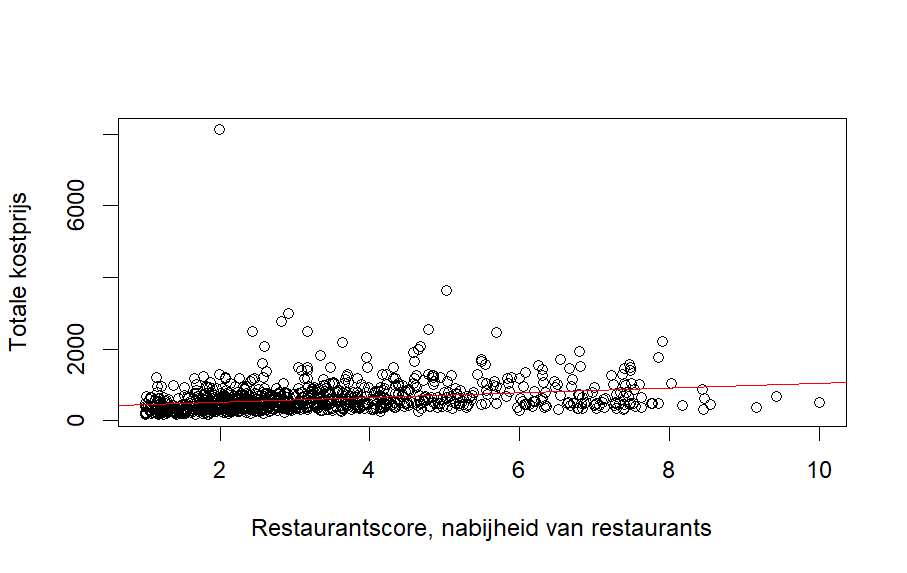
\includegraphics[width=0.49\linewidth]{../../../../Pictures/project.stat/rest}
	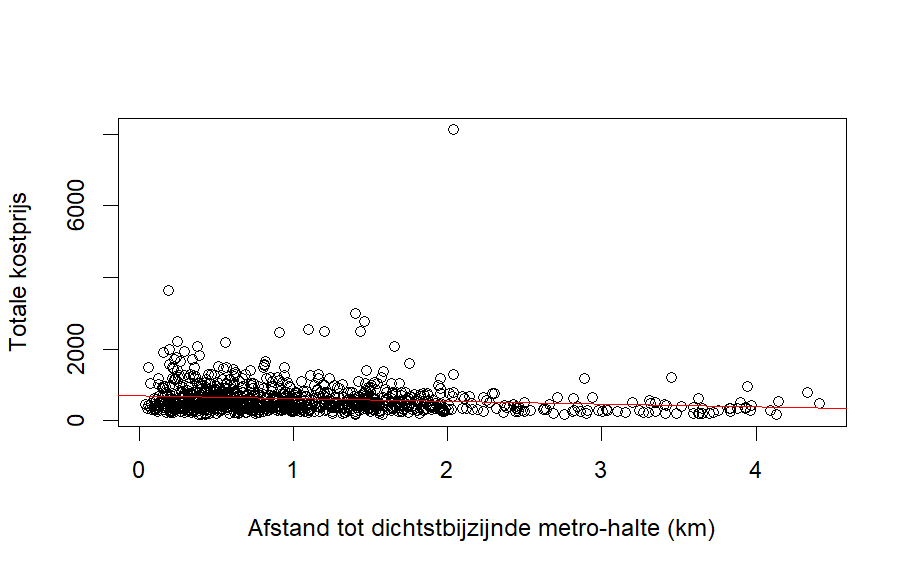
\includegraphics[width=0.49\linewidth]{../../../../Pictures/project.stat/metro}
	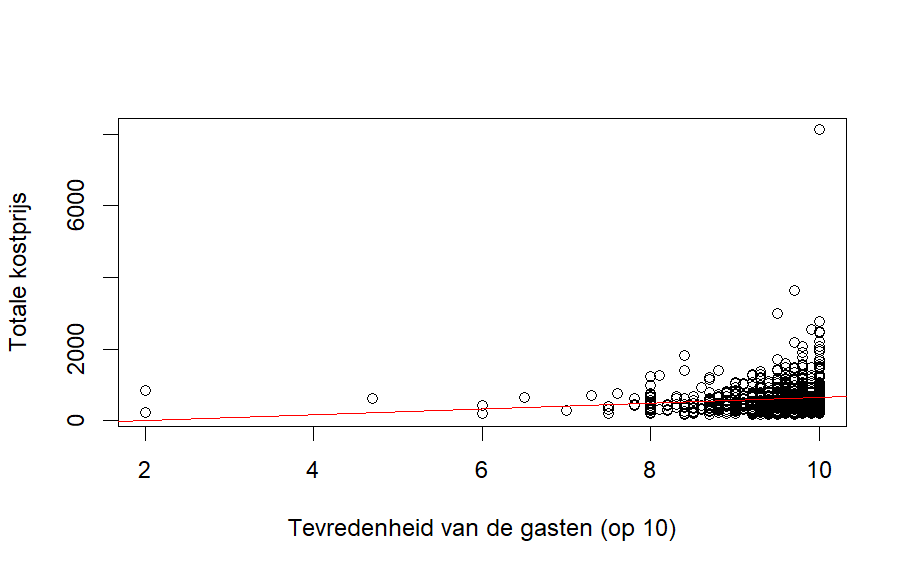
\includegraphics[width=0.49\linewidth]{../../../../Pictures/project.stat/satis}
	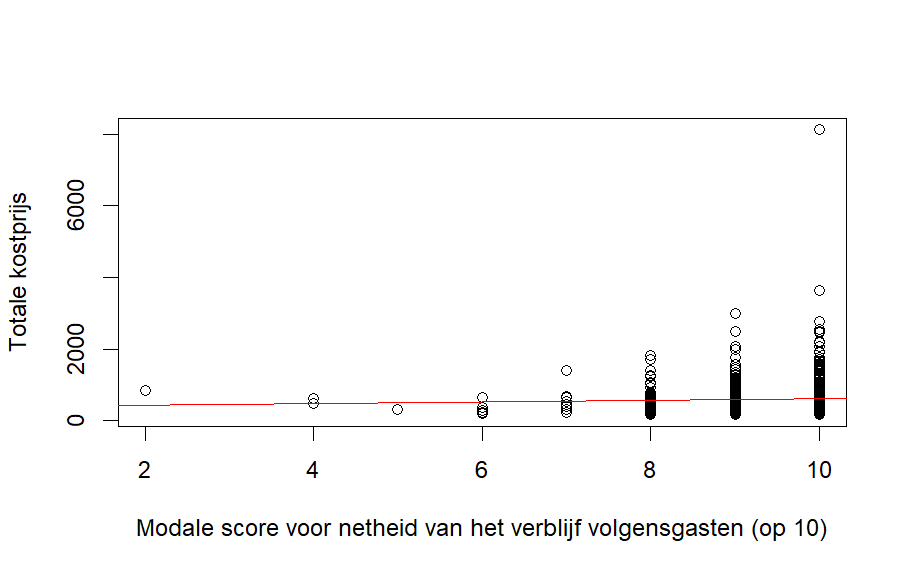
\includegraphics[width=0.49\linewidth]{../../../../Pictures/project.stat/cleanliness}
	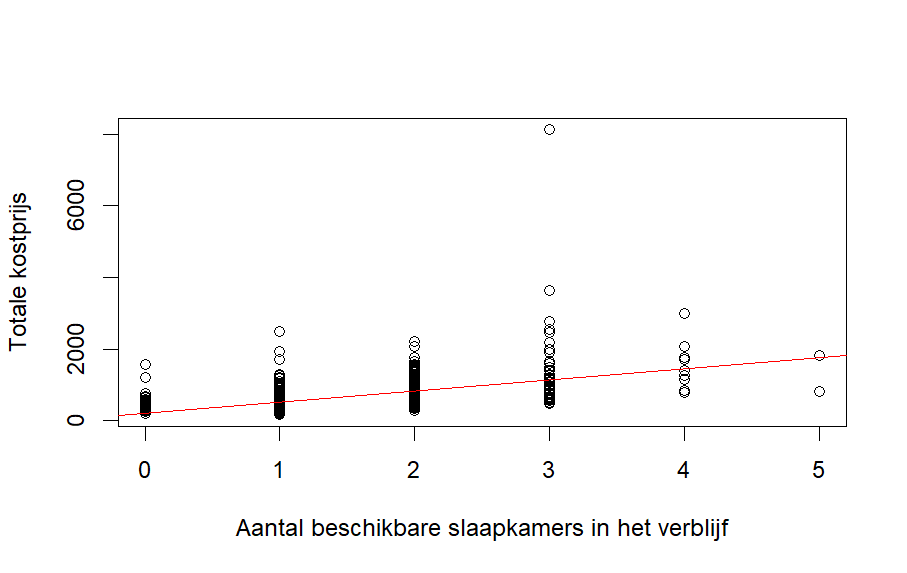
\includegraphics[width=0.49\linewidth]{../../../../Pictures/project.stat/bedrooms}
	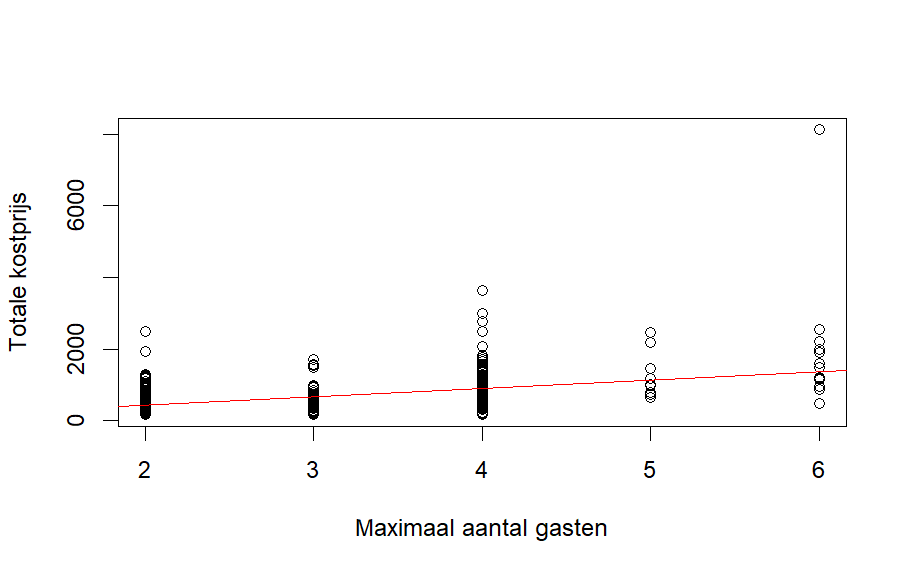
\includegraphics[width=0.49\linewidth]{../../../../Pictures/project.stat/capacity}
	\caption{Scatterplots voor de totale prijs in functie van de andere veranderlijken}
	\label{fig:scatter}
\end{figure}
	\subsection{Verklaren van de kost}
	
	
	\section*{Besluit}
	%hebben we deze tabel ergens nodig?
	\begin{table}[h]
		\begin{tabular}{r*{2}{|r}}
			Veranderlijke & Uitkomst 1 & Uitkomst 2 \\ \hline
			Aantal &            &            \\ \hline
			Proportie &            &
		\end{tabular}
	\end{table}
\end{document} 